\documentclass{article}

% 中文支持
\usepackage[UTF8]{ctex}

% 数学公式支持
\usepackage{amsmath, amssymb}

% 页边距设置
\usepackage[margin=1in]{geometry}

% 禁止浮动
\usepackage{float}

% 插图支持
\usepackage{graphicx}
\graphicspath{{./figures/word/}}

% 标题信息
\title{高维语义空间对齐与概念漂移：词级分析}
\author{陈伊凡}
\date{\today}

\begin{document}

\maketitle

\section{问题形式化}

设 $X_{\text{all}} \in \mathbb{R}^{n \times d}$ 为基于人民日报语料训练的词向量矩阵，$Y_{\text{all}} \in \mathbb{R}^{n \times d}$ 为基于微博语料训练的词向量矩阵，其中 $n$ 为共有词汇数量，$d = 300$ 为向量维度。尽管两个矩阵维度一致，但因训练过程中的随机初始化差异，二者的坐标系存在未知旋转变换。若直接比较同一词汇在两个矩阵中的坐标，将产生系统性偏差。

为解决这一问题，需先求得一个正交矩阵 $Q \in \mathbb{R}^{d \times d}$（满足 $Q^T Q = I$），将 $X_{\text{all}}$ 旋转至与 $Y_{\text{all}}$ 一致的坐标系，使得同一词汇的跨语料向量在该坐标系下具备可比性。这一过程称为正交普鲁克分析。

\section{正交普鲁克分析}

\subsection{优化目标}

选取 $m$ 个锚点词（$m \ll n$），记其在人民日报中的向量矩阵为 $X \in \mathbb{R}^{m \times d}$，在微博中的向量矩阵为 $Y \in \mathbb{R}^{m \times d}$。目标为求解正交矩阵 $Q$，最小化旋转后矩阵与目标矩阵之间的 Frobenius 范数平方：
\[
\min_{Q} \| XQ - Y \|_F^2 \quad \text{s.t.} \quad Q^T Q = I
\]

\subsection{目标化简与 SVD 求解}

将 Frobenius 范数展开，利用迹的循环性质 $\text{tr}(AB) = \text{tr}(BA)$ 及正交约束 $QQ^T = I$，可将目标函数中与 $Q$ 无关的常数项分离。化简后，原最小化问题等价于最大化 $\text{tr}(Q^T X^T Y)$。

令 $M = X^T Y \in \mathbb{R}^{d \times d}$，对 $M$ 进行奇异值分解：
\[
M = U \Sigma V^T
\]
其中 $U, V \in \mathbb{R}^{d \times d}$ 为正交矩阵，$\Sigma = \text{diag}(\sigma_1, \sigma_2, \dots, \sigma_d)$ 为对角矩阵，且奇异值 $\sigma_i \geq 0$。

代入目标函数：
\[
\text{tr}(Q^T M) = \text{tr}(Q^T U \Sigma V^T) = \text{tr}(V^T Q^T U \Sigma)
\]
令 $Z = V^T Q^T U$，由于 $V, Q, U$ 均为正交矩阵，其乘积 $Z$ 仍为正交矩阵，即 $Z^T Z = I$。于是问题转化为：
\[
\max_{Z} \text{tr}(Z \Sigma) \quad \text{s.t.} \quad Z^T Z = I
\]
由于 $\Sigma$ 为对角矩阵，$\text{tr}(Z \Sigma) = \sum_{i=1}^{d} z_{ii} \sigma_i$。对于正交矩阵 $Z$，其对角线元素满足 $|z_{ii}| \leq 1$。要使得加权和最大，应令所有 $z_{ii} = 1$，此时 $Z = I$。

由 $Z = I$ 倒推得最优旋转矩阵 $Q = U V^T$。对齐后的全量人民日报词向量矩阵为 $X_{\text{aligned}} = X_{\text{all}} Q$。该变换是正交变换，向量间距离和夹角保持不变，语义空间的内部几何结构得以保留。

\subsection{对齐质量评估}

在利用对齐后的空间进行语义漂移计算之前，需对旋转矩阵 $Q$ 进行严格验证。

\textbf{正交性验证。}
计算 $Q^T Q$ 与单位矩阵 $I$ 的最大绝对误差。实验表明，该误差为 $1.19 \times 10^{-6}$，远小于 $10^{-5}$，确认 $Q$ 为正交矩阵，变换仅包含旋转和反射，未引入拉伸或扭曲。

\textbf{距离改善率。}
为消除向量长度对欧氏距离的影响，先对锚点词向量做 L2 归一化，再计算对齐前后的欧氏距离变化。使用 A 同学选取的 2500 个高频实词作为验证集，对齐后平均欧氏距离从 0.8655 降至 0.8536，改善率为 0.7\%。同时，对齐后平均余弦相似度从 0.6187 升至 0.6329，方向一致性有所提高。

\textbf{功能词与实词验证对比。}
当改用 40 个语义绝对稳定的功能词（的、一、是、了、在、和、也、有等）作为验证锚点时，距离改善率达 18.3\%，显著高于 2500 个实词的 0.7\%。这一差异并非对齐失败，而是实词在两个语料中天然存在语义差异——例如"覆盖"在新闻中指信号覆盖，在微博中指积雪覆盖，这部分差异无法也不应该通过旋转消除。功能词验证的高改善率证明对齐本身是有效的，实词的低改善率恰好从侧面印证了跨语料实词语义差异的客观存在。

\section{语义漂移的量化}

\subsection{余弦相似度与漂移量}

对于任意词汇 $w$，设对齐后的旧向量为 $\vec{v}_{\text{old}} \in \mathbb{R}^d$，新向量为 $\vec{v}_{\text{new}} \in \mathbb{R}^d$。两者的余弦相似度定义为：
\[
\cos(\theta) = \frac{\vec{v}_{\text{old}} \cdot \vec{v}_{\text{new}}}{\|\vec{v}_{\text{old}}\|_2 \cdot \|\vec{v}_{\text{new}}\|_2}
\]
值域为 $[-1, 1]$，越接近 $1$ 表示两向量方向越一致。

定义词汇 $w$ 的语义漂移量为：
\[
\text{Shift}(w) = 1 - \cos(\theta)
\]
漂移量越大，表示该词汇在两个语料中的语义变化越显著。理论上值域为 $[0, 2]$，实际观测到的语义变化通常在 $[0, 0.5]$ 之间。

\subsection{最近邻重排}

除直接计算词向量本身的位移外，还可通过考察词汇"邻居"的变化来度量语义漂移。对于任意词汇 $w$，分别在对齐后的空间 $X_{\text{aligned}}$ 和 $Y_{\text{all}}$ 中找出其 $k$ 个最近邻，记旧空间中的邻居集合为 $N_{\text{old}}(w)$，新空间中的邻居集合为 $N_{\text{new}}(w)$。两集合的相似程度用 Jaccard 相似度衡量：
\[
J(w) = \frac{|N_{\text{old}}(w) \cap N_{\text{new}}(w)|}{|N_{\text{old}}(w) \cup N_{\text{new}}(w)|}
\]
$J(w) \approx 1$ 表示邻居基本不变，语义环境稳定；$J(w) \approx 0$ 表示邻居几乎完全更换，语义环境发生剧烈变化。所有词汇的平均 Jaccard 值定义为局部邻域稳定性，从宏观上衡量语义空间的局部结构保持程度。

\section{统计显著性检验}

为区分真实的语义变化与随机波动，选取 40 个公认语义稳定的高频功能词（的、一、是、了、我、不、在、人、他、有、这、个、们、中、来、上、大、为、就、和、说、地、也、对、到、要、下、会、时、出、那、过、你、她、能、前、它、所、都、后）作为锚点词集合，计算其漂移量分布。40 个锚点词的平均漂移量为 0.48，标准差为 0.085。以均值加两倍标准差（$\mu + 2\sigma$）作为统计显著性阈值，即 0.65。若某词汇的漂移量超过该阈值，则判定其语义变化具有统计显著性。

锚点词集合承担双重功能：一是作为参照组建立统计显著性基线，二是在普鲁克分析中参与对齐过程。二者在逻辑上独立——前者利用锚点词的实际漂移量分布评估其他词的变化是否超出正常范围，后者基于锚点词语义绝对稳定的假设求解旋转矩阵 $Q$。

\section{数据预处理}

\subsection{数据来源}

本实验使用两组中文词向量：人民日报词向量基于 1946--2017 年新闻语料训练，代表传统正式语境；微博词向量基于新浪微博社交媒体语料训练，代表网络非正式语境。两组词向量均为 300 维，训练方法为 Skip-Gram with Negative Sampling（SGNS）。原始共有词汇约 13.9 万条。

\subsection{清洗策略}

采用分层清洗策略。锚点词从原始共有词中选取 40 个功能词，允许单字，因为功能词语义绝对稳定且需在共有词中普遍存在。非锚点词严格过滤标点、数字、英文及乱码，仅保留长度 $\geq 2$ 的纯中文词，取词频最高的 5000 个用于漂移量计算。A 同学独立选取了 2500 个高频实词（纯中文、长度 $\geq 2$）作为普鲁克分析的锚点集合，用于求解旋转矩阵 $Q$。

\subsection{清洗的必要性}

未经清洗时，漂移量 Top 20 被标点符号、数字和乱码占据；清洗后转变为具有语义解释力的词汇。但低频人名地名仍占据 Top 20——它们在两个语料中出现频率极低，训练不充分，向量方向本身具有较大随机性，漂移量虚高是静态词向量的固有限制。

\section{词级分析结果}

\subsection{锚点词漂移量与基线}

40 个锚点词的漂移量分布如下：平均值为 0.48，标准差为 0.085，个体取值在 0.31（"她"）至 0.66（"我"）之间。据此确定显著性阈值为 $\mu + 2\sigma = 0.65$。

\subsection{漂移量分布}

5000 个高频非锚点词的漂移量整体集中在 0.3--0.7 之间，分布呈右偏态，少数词汇超过阈值。

\begin{figure}[H]
\centering
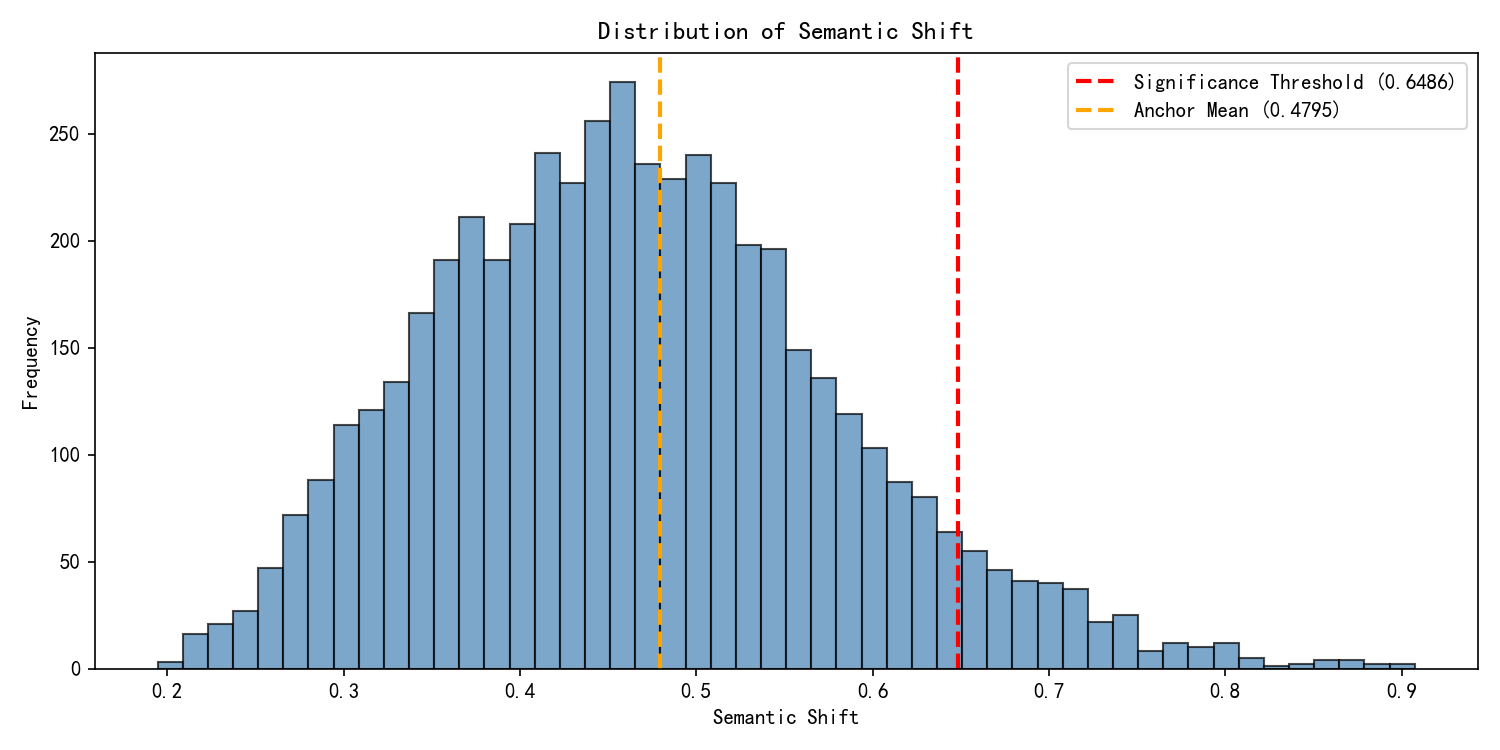
\includegraphics[width=0.9\textwidth]{shift_distribution.png}
\caption{5000 个高频非锚点词的漂移量分布直方图}
\label{fig:dist}
\end{figure}

如图 \ref{fig:dist} 所示，红色虚线为显著性阈值（0.65），橙色虚线为锚点词均值（0.48）。大多数词汇的漂移量低于阈值，说明多数高频词在两种语料中的语义保持相对稳定。

\subsection{自动 Top 20 与人名噪声}

自动生成的漂移量 Top 20 如下图所示：

\begin{figure}[H]
\centering
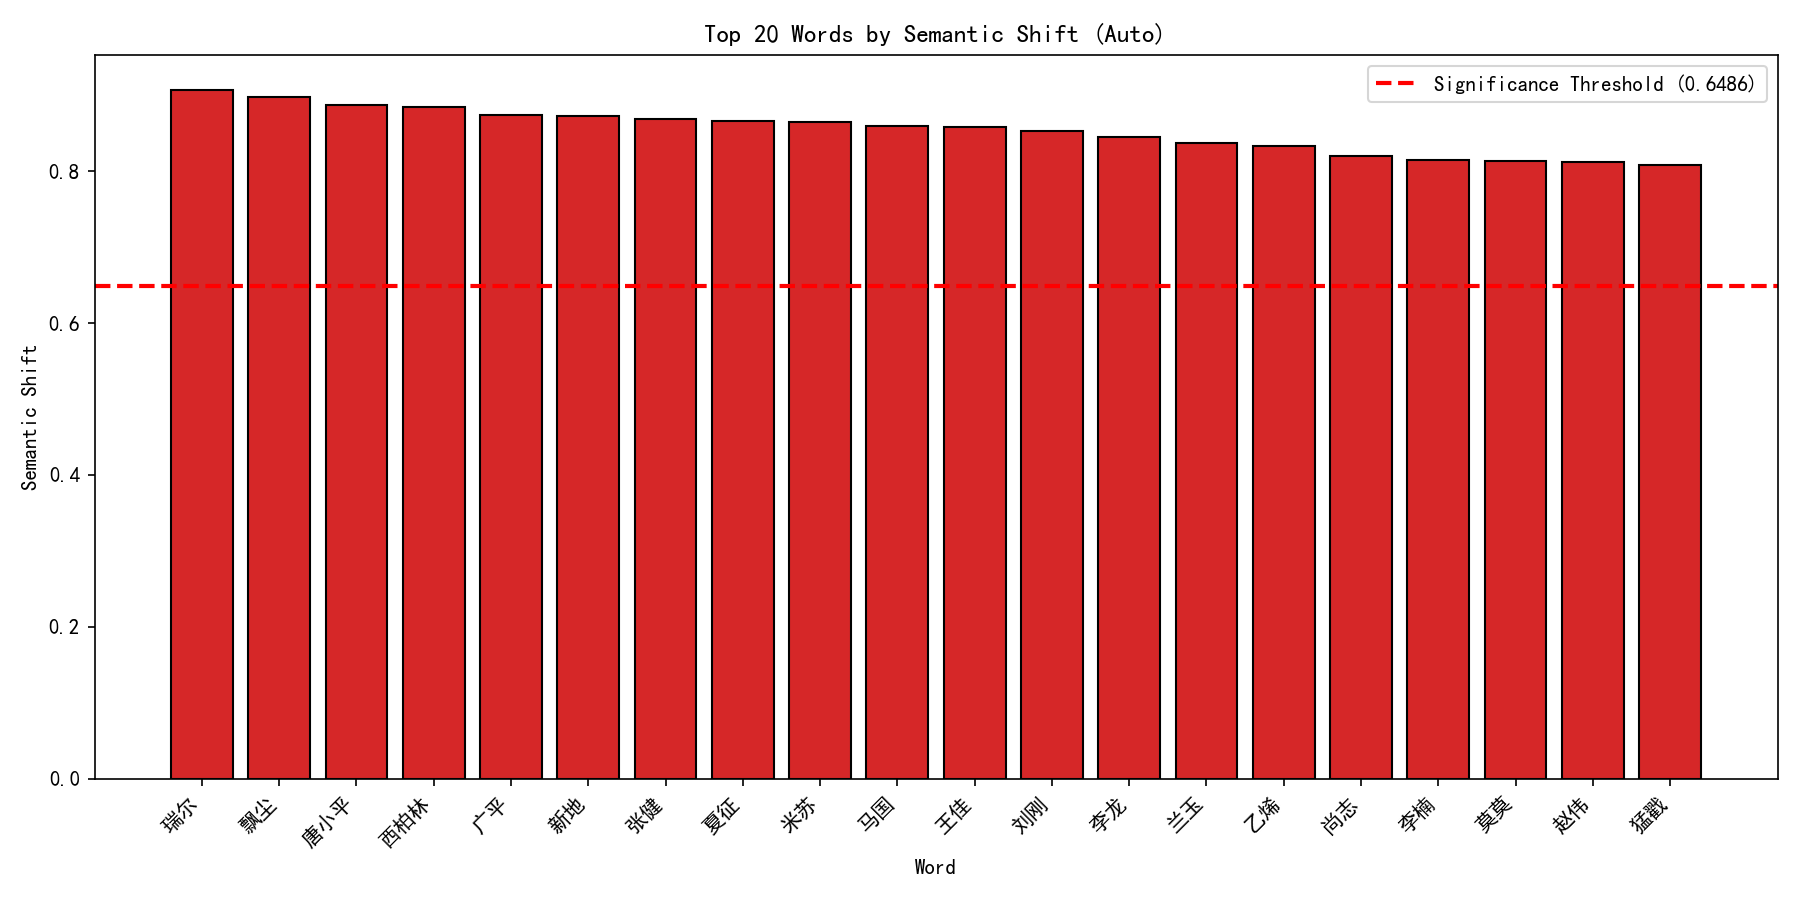
\includegraphics[width=0.9\textwidth]{shift_top20_auto.png}
\caption{语义漂移量 Top 20（自动生成）}
\label{fig:auto}
\end{figure}

如图 \ref{fig:auto} 所示，Top 20 全部为罕见人名、地名和专有名词，漂移量在 0.80--0.91 之间，均超过显著性阈值。这些词在两个语料中均为低频词，训练不充分，向量方向具有较大随机性，漂移量虚高是静态词向量在低频词上的固有限制，不能等同于真正的语义漂移。

\subsection{人工精选高价值漂移词}

为提取真正有语义变化信号的词汇，从漂移量 Top 200 中手工筛选，排除低频专有名词后精选了 20 个高价值词：

\begin{figure}[H]
\centering
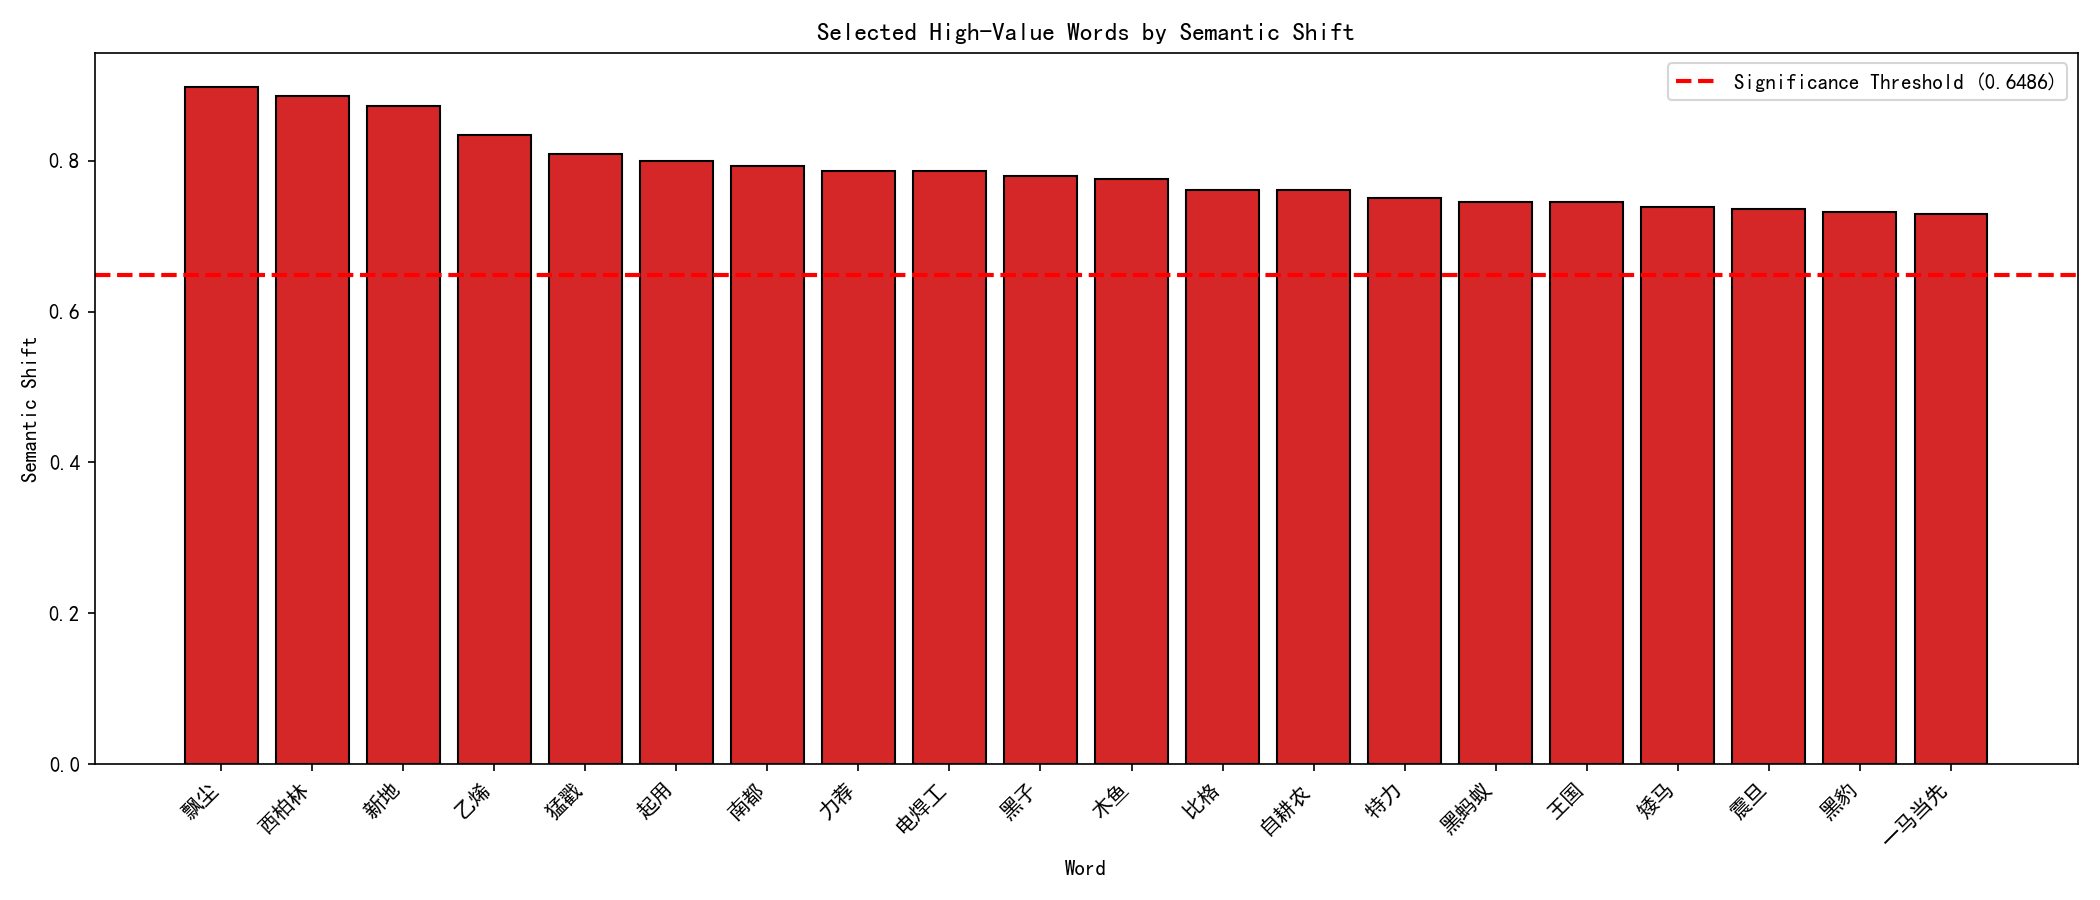
\includegraphics[width=0.95\textwidth]{shift_top20_selected.png}
\caption{人工精选高价值漂移词}
\label{fig:selected}
\end{figure}

如图 \ref{fig:selected} 所示，精选词包括"乙烯"（化工原料，新闻工业语境 vs 微博日常语境）、"猛戳"（网络用语，新闻中几乎不出现）、"电焊工"（职业名词，新闻正式称谓 vs 微博口语化表达）、"南都"（媒体简称，新闻高频 vs 微博低频）、"黑子"（网络用语，指恶意批评者）、"一马当先"（成语，新闻常用 vs 微博罕见）等。这些词的跨语料差异反映了人民日报与微博在话题覆盖和用词风格上的系统性区别。

\subsection{语义稳定词}

漂移量最低的 20 个词以专业术语和医学词汇为主（如罗马式、多糖类、血管收缩等），漂移量在 0.15--0.21 之间。需要指出的是，这些词漂移量低主要因为它们在两个语料中均为低频词，训练不充分导致向量本身就带有较大随机性，表现为"伪稳定"现象。

\subsection{最近邻重排}

在不同 $k$ 值下计算的平均 Jaccard 相似度如下：$k=10$ 时平均 Jaccard 为 0.0904，$k=50$ 时为 0.1602。$k=10$ 时 Jaccard 仅约 0.09，说明在严格局部邻域层面，同一个词在人民日报和微博中的"邻居圈子"几乎完全不同——10 个邻居中平均不到 1 个保留。扩大至 $k=50$ 后，平均 Jaccard 上升至 0.16，表明在更宽松的邻域范围内仍存在少量结构延续。这一结果从局部语义结构的视角，独立验证了两种语料之间确实存在系统性的语义差异。

\section{误差来源与局限性}

\textbf{低频词与罕见专有名词。}
漂移量 Top 20 中大量罕见人名地名是静态词向量的固有限制。这类词在两个语料中出现频率极低，训练不充分，向量方向本身带有较大随机性，漂移量虚高。通过人工筛选从 Top 200 中提取高价值漂移词可规避此问题，但无法从根本上解决低频词噪声。

\textbf{语料主题差异。}
人民日报语料以政治、历史、外交等严肃新闻为主，微博语料以生活、娱乐、社交等日常话题为主。观测到的"语义漂移"部分源于两个语料的主题分布差异，在解读时应将其理解为"跨语料语义差异"而非严格的"历时语义变化"。

\textbf{锚点词选择的两难。}
普鲁克分析需要覆盖面广、方向明确的实词作为锚点以求准旋转矩阵 $Q$；而统计检验需要语义绝对稳定的功能词作为基线。A 同学用 2500 个实词求 $Q$，本研究用 40 个功能词建基线，两批词各司其职。这一分层策略在逻辑上自洽，但两种锚点之间的差异（功能词改善率 18.3\% vs 实词 0.7\%）也说明实词的跨语料语义差异是真实存在的，无法也不应通过旋转消除。

\textbf{静态词向量的固有限制。}
本研究所用词向量为静态表示（SGNS），每个词仅有一个固定向量，无法区分多义词的不同义项。上下文相关的动态词向量（如 BERT）可提供更细粒度的语义表示，是后续研究的重要方向。

\end{document}